\documentclass{article}
\usepackage[final]{nips_2017}
\usepackage[polish]{babel}
\usepackage[utf8]{inputenc} % allow utf-8 input
\usepackage[T1]{fontenc}    % use 8-bit T1 fonts
\usepackage{hyperref}       % hyperlinks
\usepackage{url}            % simple URL typesetting
\usepackage{booktabs}       % professional-quality tables
\usepackage{amsfonts}       % blackboard math symbols
\usepackage{nicefrac}       % compact symbols for 1/2, etc.
\usepackage{microtype}      % microtypography
\usepackage{graphicx}
\usepackage[section]{placeins}
\graphicspath{ {./images/} }

\title{ Sieć wielowarstwowa uczona metodą propagacji wstecznej  }

\author{
  Autor: Rafał Behrendt \\
  \texttt{246643@student.pwr.edu.pl} \\
  Prowadząca: dr hab. inż. Urszula Markowska-Kaczmar \\
  \today
}

\begin{document}

\maketitle

\begin{abstract}
  Celem ćwiczenia jest zapoznanie się z siecią wielowarstwową, uczeniem sieci za 
  pomocą algorytmu propagacji wstecznej w wersji klasycznej (minimalizacja błędu) 
  średniokwadratowego oraz wpływem parametrów odgrywających istotną rolę w uczeniu 
  sieci z propagacją wsteczną. Eksperymenty przeprowadzono na zbiorze MNIST zawierającym 60000 danych treningowych
  oraz 10000 danych testowych.
\end{abstract}

Kod źródłowy znajduje się w poniższym linku:

\begin{center}
  \url{https://github.com/aspirew/neuralNetworks/tree/list2}
\end{center}

\newpage
\section{Eksperymenty}

Za domyślne hiperparametry przyjęto:

\begin{itemize}
  \item Wielkość sieci: [20]
  \item Współczynnik uczenia: 0.3
  \item Funkcja aktywacji: tangens hiperboliczy
  \item Inicjalizacja wag za pomocą rozkładu normalnego o parametrach:
  \subitem mi: 0
  \subitem sigma: 0.5
\end{itemize}

Każdy test przeszedł przez 50 epok zanim został zakończony.

\subsection{Test wielkości sieci}

Zbadano jak wielkości sieci - liczba warstw wraz z liczbą neuronów w warstwach wpływa na skuteczność i szybkość uczenia.
Zapis [5, 7] oznacza sieć neuronową z dwoma warstwami ukrytmi, z czego pierwsza zawiera 5 neuronów, a druga 7.
Ilość neuronów na wyjściu wynosi zawsze 10. W tabelce zawarty jest uśredniony błąd oraz oraz uśredniona liczba prawidłowo rozpoznanych
liczb ze zbioru testowego. Niżej przedstawione są wyniki na wykresach.

\begin{table}[h]
  \centering
    
  \bgroup
  \def\arraystretch{1.3}
\begin{tabular}{|l|l|l|}
\hline
Wielkość & Błąd & Skuteczność \\ \hline
{[}5{]} & 0.478 & 8594 \\ \hline
{[}10{]} & 0.27 & 9176 \\ \hline
{[}20{]} & 0.15 & 9374 \\ \hline
{[}30{]} & 0.11 & 9496 \\ \hline
{[}5, 5{]} & 0.5 & 8548 \\ \hline
{[}5, 10, 20{]} & 0.45 & 8659 \\ \hline
\end{tabular}
  \egroup
  \vspace{10pt}
  \caption{Wielkość sieci}
\end{table}

\begin{figure}[]
  \centering
  \includegraphics[width=\linewidth]{hiddenLayer/error_hidden_layer_[5].png}
\end{figure}

\begin{figure}[]
  \centering
  \includegraphics[width=\linewidth]{hiddenLayer/passedTest_learn_rate_[5].png}
\end{figure}

\begin{figure}[]
  \centering
  \includegraphics[width=\linewidth]{hiddenLayer/error_hidden_layer_[10].png}
\end{figure}

\begin{figure}[]
  \centering
  \includegraphics[width=\linewidth]{hiddenLayer/passedTest_learn_rate_[10].png}
\end{figure}

\begin{figure}[]
  \centering
  \includegraphics[width=\linewidth]{hiddenLayer/error_hidden_layer_[20].png}
\end{figure}

\begin{figure}[]
  \centering
  \includegraphics[width=\linewidth]{hiddenLayer/passedTest_learn_rate_[20].png}
\end{figure}

\begin{figure}[]
  \centering
  \includegraphics[width=\linewidth]{hiddenLayer/error_hidden_layer_[30].png}
\end{figure}

\begin{figure}[]
  \centering
  \includegraphics[width=\linewidth]{hiddenLayer/passedTest_learn_rate_[30].png}
\end{figure}

\begin{figure}[]
  \centering
  \includegraphics[width=\linewidth]{hiddenLayer/error_hidden_layer_[5, 5].png}
\end{figure}

\begin{figure}[]
  \centering
  \includegraphics[width=\linewidth]{hiddenLayer/passedTest_learn_rate_[5, 5].png}
\end{figure}

\begin{figure}[]
  \centering
  \includegraphics[width=\linewidth]{hiddenLayer/error_hidden_layer_[5, 10, 20].png}
\end{figure}

\begin{figure}[]
  \centering
  \includegraphics[width=\linewidth]{hiddenLayer/passedTest_learn_rate_[5, 10, 20].png}
\end{figure}


\newpage
\subsection{Test wielkości współczynnika uczenia}

Zbadano jak współczynnik uczenia wpływa na spadek błędu i skuteczność sieci. W tabelce zawarty jest uśredniony błąd oraz oraz uśredniona liczba prawidłowo rozpoznanych
liczb ze zbioru testowego. Niżej przedstawione są wyniki na wykresach.

\begin{table}[h]
  \centering
    
  \bgroup
  \def\arraystretch{1.3}
  \begin{tabular}{|l|l|l|}
  \hline
  Współczynnik uczenia & Błąd & Skuteczność \\ \hline
  {0.01} & 0.478 & 8594 \\ \hline
  {0.05} & 0.27 & 9176 \\ \hline
  {0.1} & 0.2 & 9309 \\ \hline
  {0.2} & 0.17 & 9320 \\ \hline
  {0.3} & 0.15 & 9401 \\ \hline
  {0.5} & 0.13 & 9441 \\ \hline
  {0.75} & 0.15 & 9395 \\ \hline
  {1} & 0.16 & 9353 \\ \hline
  \end{tabular}
  \egroup
  \vspace{10pt}
  \caption{Współczynnik uczenia}
\end{table}

\newpage
\begin{figure}[!htb]
  \centering
  \includegraphics[width=\linewidth]{learnRate/error_learn_rate_0.01.png}
\end{figure}

\begin{figure}[!htb]
  \centering
  \includegraphics[width=\linewidth]{learnRate/test_learn_rate_0.01.png}
\end{figure}

\begin{figure}[]
  \centering
  \includegraphics[width=\linewidth]{learnRate/error_learn_rate_0.05.png}
\end{figure}

\begin{figure}[]
  \centering
  \includegraphics[width=\linewidth]{learnRate/test_learn_rate_0.05.png}
\end{figure}

\begin{figure}[]
  \centering
  \includegraphics[width=\linewidth]{learnRate/error_learn_rate_0.1.png}
\end{figure}

\begin{figure}[]
  \centering
  \includegraphics[width=\linewidth]{learnRate/test_learn_rate_0.1.png}
\end{figure}

\begin{figure}[]
  \centering
  \includegraphics[width=\linewidth]{learnRate/error_learn_rate_0.2.png}
\end{figure}

\begin{figure}[]
  \centering
  \includegraphics[width=\linewidth]{learnRate/test_learn_rate_0.2.png}
\end{figure}

\begin{figure}[]
  \centering
  \includegraphics[width=\linewidth]{learnRate/error_learn_rate_0.3.png}
\end{figure}

\begin{figure}[]
  \centering
  \includegraphics[width=\linewidth]{learnRate/test_learn_rate_0.3.png}
\end{figure}

\begin{figure}[]
  \centering
  \includegraphics[width=\linewidth]{learnRate/error_learn_rate_0.5.png}
\end{figure}

\begin{figure}[]
  \centering
  \includegraphics[width=\linewidth]{learnRate/test_learn_rate_0.5.png}
\end{figure}

\begin{figure}[]
  \centering
  \includegraphics[width=\linewidth]{learnRate/error_learn_rate_0.75.png}
\end{figure}

\begin{figure}[]
  \centering
  \includegraphics[width=\linewidth]{learnRate/test_learn_rate_0.75.png}
\end{figure}

\begin{figure}[]
  \centering
  \includegraphics[width=\linewidth]{learnRate/error_learn_rate_1.png}
\end{figure}

\begin{figure}[]
  \centering
  \includegraphics[width=\linewidth]{learnRate/test_learn_rate_1.png}
\end{figure}


\newpage
\subsection{Test wielkości paczki}

Zbadano jak wielkość paczki wpływa na spadek błędu i skuteczność sieci. W tabelce zawarty jest uśredniony błąd oraz oraz uśredniona liczba prawidłowo rozpoznanych
liczb ze zbioru testowego. Niżej przedstawione są wyniki na wykresach.

\begin{table}[h]
  \centering
    
  \bgroup
  \def\arraystretch{1.3}
  \begin{tabular}{|l|l|l|l|}
  \hline
  Wielkość paczki & Błąd & Skuteczność \\ \hline
  10 & 0.15 & 9440 \\ \hline
  50 & 0.15 & 9400 \\ \hline
  100 & 0.19 & 9312 \\ \hline
  500 & 0.31 & 9053 \\ \hline
  1000 & 0.39 & 8893 \\ \hline
  10000 & 0.39 & 8884 \\ \hline
  60000 & 0.38 & 8902 \\ \hline
  \end{tabular}
  \egroup
  \vspace{10pt}
  \caption{Wielkość paczki}
\end{table}

\newpage
\begin{figure}[!htb]
  \centering
  \includegraphics[width=\linewidth]{batchSize/error_batch_size_10.png}
\end{figure}

\begin{figure}[!htb]
  \centering
  \includegraphics[width=\linewidth]{batchSize/test__batch_size_10.png}
\end{figure}

\begin{figure}[]
  \centering
  \includegraphics[width=\linewidth]{batchSize/error_batch_size_50.png}
\end{figure}

\begin{figure}[]
  \centering
  \includegraphics[width=\linewidth]{batchSize/test__batch_size_50.png}
\end{figure}

\begin{figure}[]
  \centering
  \includegraphics[width=\linewidth]{batchSize/error_batch_size_100.png}
\end{figure}

\begin{figure}[]
  \centering
  \includegraphics[width=\linewidth]{batchSize/test__batch_size_100.png}
\end{figure}

\begin{figure}[]
  \centering
  \includegraphics[width=\linewidth]{batchSize/error_batch_size_500.png}
\end{figure}

\begin{figure}[]
  \centering
  \includegraphics[width=\linewidth]{batchSize/test__batch_size_500.png}
\end{figure}

\begin{figure}[]
  \centering
  \includegraphics[width=\linewidth]{batchSize/error_batch_size_1000.png}
\end{figure}

\begin{figure}[]
  \centering
  \includegraphics[width=\linewidth]{batchSize/test__batch_size_1000.png}
\end{figure}

\begin{figure}[]
  \centering
  \includegraphics[width=\linewidth]{batchSize/error_batch_size_2000.png}
\end{figure}

\begin{figure}[]
  \centering
  \includegraphics[width=\linewidth]{batchSize/test__batch_size_2000.png}
\end{figure}

\begin{figure}[]
  \centering
  \includegraphics[width=\linewidth]{batchSize/error_batch_size_60000.png}
\end{figure}

\begin{figure}[]
  \centering
  \includegraphics[width=\linewidth]{batchSize/test__batch_size_60000.png}
\end{figure}

\newpage
\subsection{Test inicjalizacji wartości wag}

Zbadano jak sposób inicjalizacji wag wpływa na spadek błędu i skuteczność sieci. Do inicjalizacji wag wykorzystano rozkład normalny.
Mediana ustawiona jest zawsze na zero, a badany jest wpływ zmiany odchylenia standardowego. 
W tabelce zawarty jest uśredniony błąd oraz oraz uśredniona liczba prawidłowo rozpoznanych
liczb ze zbioru testowego. Niżej przedstawione są wyniki na wykresach.

\begin{table}[h]
  \centering
    
  \bgroup
  \def\arraystretch{1.3}
  \begin{tabular}{|l|l|l|l|}
  \hline
  Sigma & Błąd & Skuteczność \\ \hline
  0.1 & 0.1 & 9504 \\ \hline
  0.2 & 0.11 & 9466 \\ \hline
  0.3 & 0.13 & 9441 \\ \hline
  0.4 & 0.13 & 9411 \\ \hline
  0.5 & 0.17 & 9332 \\ \hline
  0.6 & 0.18 & 9312 \\ \hline
  0.7 & 0.2 & 9281 \\ \hline
  0.8 & 0.22 & 9271 \\ \hline
  0.9 & 0.24 & 9155 \\ \hline
  1 & 0.27 & 9146 \\ \hline
  \end{tabular}
  \egroup
  \vspace{10pt}
  \caption{Wielkość odchylenia standardowego}
\end{table}

\newpage
\begin{figure}[!htb]
  \centering
  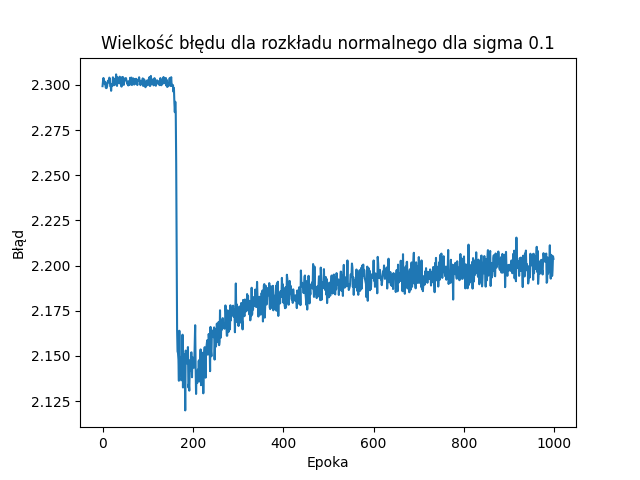
\includegraphics[width=\linewidth]{weight/error_weight_0.1.png}
\end{figure}

\begin{figure}[!htb]
  \centering
  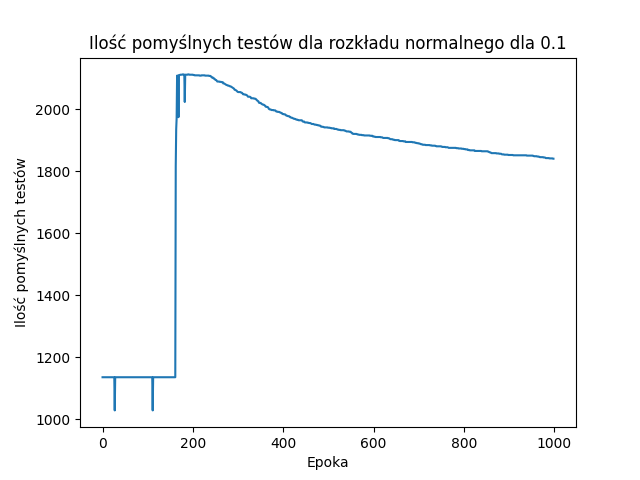
\includegraphics[width=\linewidth]{weight/test_weight_0.1.png}
\end{figure}

\begin{figure}[]
  \centering
  \includegraphics[width=\linewidth]{weight/error_weight_0.2.png}
\end{figure}

\begin{figure}[]
  \centering
  \includegraphics[width=\linewidth]{weight/test_weight_0.2.png}
\end{figure}

\begin{figure}[]
  \centering
  \includegraphics[width=\linewidth]{weight/error_weight_0.3.png}
\end{figure}

\begin{figure}[]
  \centering
  \includegraphics[width=\linewidth]{weight/test_weight_0.3.png}
\end{figure}

\begin{figure}[]
  \centering
  \includegraphics[width=\linewidth]{weight/error_weight_0.4.png}
\end{figure}

\begin{figure}[]
  \centering
  \includegraphics[width=\linewidth]{weight/test_weight_0.4.png}
\end{figure}

\begin{figure}[]
  \centering
  \includegraphics[width=\linewidth]{weight/error_weight_0.5.png}
\end{figure}

\begin{figure}[]
  \centering
  \includegraphics[width=\linewidth]{weight/test_weight_0.5.png}
\end{figure}

\begin{figure}[]
  \centering
  \includegraphics[width=\linewidth]{weight/error_weight_0.6.png}
\end{figure}

\begin{figure}[]
  \centering
  \includegraphics[width=\linewidth]{weight/test_weight_0.6.png}
\end{figure}

\begin{figure}[]
  \centering
  \includegraphics[width=\linewidth]{weight/error_weight_0.7.png}
\end{figure}

\begin{figure}[]
  \centering
  \includegraphics[width=\linewidth]{weight/test_weight_0.7.png}
\end{figure}

\begin{figure}[]
  \centering
  \includegraphics[width=\linewidth]{weight/error_weight_0.8.png}
\end{figure}

\begin{figure}[]
  \centering
  \includegraphics[width=\linewidth]{weight/test_weight_0.8.png}
\end{figure}

\begin{figure}[]
  \centering
  \includegraphics[width=\linewidth]{weight/error_weight_0.9.png}
\end{figure}

\begin{figure}[]
  \centering
  \includegraphics[width=\linewidth]{weight/test_weight_0.9.png}
\end{figure}

\begin{figure}[]
  \centering
  \includegraphics[width=\linewidth]{weight/error_weight_1.0.png}
\end{figure}

\begin{figure}[]
  \centering
  \includegraphics[width=\linewidth]{weight/test_weight_1.0.png}
\end{figure}


\subsection{Test funkcji aktywacji}

W sieci neuronowej przetestowano 3 różne funkcje aktywacji: sigmoidalną, tangensa hiperbolicznego oraz softplus.
W tabelce zawarty jest uśredniony błąd oraz oraz uśredniona liczba prawidłowo rozpoznanych
liczb ze zbioru testowego. Niżej przedstawione są wyniki na wykresach.

\begin{table}[h]
  \centering
    
  \bgroup
  \def\arraystretch{1.3}
  \begin{tabular}{|l|l|l|l|}
  \hline
  Funkcja aktywacji & Błąd & Skuteczność \\ \hline
  sigmoid & 0.65 & 8021 \\ \hline
  tanh & 0.17 & 9380 \\ \hline
  softplus & 0.24 & 9270 \\ \hline
  \end{tabular}
  \egroup
  \vspace{10pt}
  \caption{Funckja aktywacji}
\end{table}

\newpage
\begin{figure}[!htb]
  \centering
  \includegraphics[width=\linewidth]{activation/error_activation_sigmoid.png}
\end{figure}

\begin{figure}[!htb]
  \centering
  \includegraphics[width=\linewidth]{activation//test_activation_sigmoid.png}
\end{figure}

\begin{figure}[]
  \centering
  \includegraphics[width=\linewidth]{activation/error_activation_tanh.png}
\end{figure}

\begin{figure}[]
  \centering
  \includegraphics[width=\linewidth]{activation/test_activation_tanh.png}
\end{figure}

\begin{figure}[]
  \centering
  \includegraphics[width=\linewidth]{activation/error_activation_softplus.png}
\end{figure}

\begin{figure}[]
  \centering
  \includegraphics[width=\linewidth]{activation/test_activation_softplus.png}
\end{figure}

\section{Wnioski}

\subsection{Wielkość sieci}

Ilość warstw ukrutych wydaje się nie wpływać znacząco na skuteczność sieci. Ilość neuronów na warstwę ma z kolei widoczny pozytywny wpływ.
Duże ilości z zwiększają rozmiary matryc i ilości działań które należy wykonać, zabierają zatem więcej czasu.

\subsection{Współczynnik uczenia}

Najlepszy wynik uzyskany został dla pośredniej wartości 0.5. Zbyt niski wynik dawał wysoki błąd, a wraz z wzrost powyżej
optymalnej wartości błąd również spadał. Niski współczynnik uczenia możę wyuczyć sieć lepiej, jednak wymaga ona przejścia przez więcej epok.
Zbyt duży współczynnik może spowodować, że sieć przeoczy optymalny punkt w któym najlepiej rozpoznaje wzorce.

\subsection{Wielkość paczki}

Testy wskazują że mniejsza wielkość paczki skutkuje poprawą wyników. Mała wielkość paczki ma za zadanie
poprawić prędkość działania sieci, za cenę wprowadzenia szumu, czyli pewnych niedokładności. Można zauważyć że dla większych wartości paczki
mimo że średni wynik jest gorszy niż te niższe, to dla każdej epoki jest on bardziej stabilny - wyniki są na jednym poziomie.

\subsection{Sposób inicjalizacji wag}

Im mniejsze odchylenie standardowe tym można zauważyć lepsze wyniki - chcemy zatem aby wartości były bliskie 0. Zbyt duże odchylenie standardowe
skutkuje mniejszą dokłądnością sieci.

\subsection{Użyta funkcja aktywacji}

Można zauważyć, że z zadanym problemem najlepiej radzi sobie funkcja tangensa hiperbolicznego. Niewiele gorzej spisuje się
funkcja softplus (użyta jako substyt funkcji ReLU). Dużą niestabilnością wykazuje się funkcja sigmoidalna.

\vspace{30pt}
Przedstawione wsnioski odnoszą się do problemu rozwiązywanego na zajęciach, czyli rozpoznawania liczb ze zbioru MIST.
Mogą one nie być uniwersalne i dla innych rodzajów problemów inne hiperparametry mogą okazać się skuteczniejsze.


\end{document}